\chapter{Método}

\todo[inline]{O capítulo todo é um resumo do CRISP-DM 1.0... fico dando \\cite em todo parágrafo? o mesmo para o capítulo sobre aprendizado de máquina}

% Por que seguir um processo?
\todo[inline]{Por que um processo?}

% Reproducibilidade/padronização/etc
\cite{ML_know} \cite{balance-anarchy} \cite{ML_debt} \cite{replicability}

O processo de aplicação de técnicas de Mineração de Dados para atender a um problema real demanda não apenas conhecimentos e execução de atividades relacionadas, estritamente, a aprendizado de máquina, mas também conhecimentos e execução de atividades relacionadas ao entendimento do problema em questão. A fim de organizar as atividades envolvidas nesse processo, foram desenvolvidas especificações de processos que orientam quais os passos devem ser seguidos para partir do entendimento de um problema e chegar a uma solução baseada em Mineração de Dados, como o CRISP-DM, o KDD e o SEMMA\cite{CRISP-DM-KDD-SEMMA}.

% Por que CRISP-DM?
\todo{por que crisp-dm}
\cite{CRISP-DM-KDD-SEMMA}

\section{Processo CRISP-DM}

% História do CRISP-DM
%% p. 1-2
CRISP-DM(CRoss-Industry Standard Process for Data Mining) é um processo de aplicação de Mineração de Dados, desenvolvido pelo CRISP-DM Special Interest Group e publicado em 2000. Foi concebido em 1996 por três empresas que utilizavam Mineração de Dados: DaimlerChrysler(à época Daimler-Benz), SPSS(à época ISL) e NCR; motivadas pela incerteza com relação à qualidade de seus trabalhos, pelo questionamento de se toda nova empresa que quisesse aplicar Mineração de Dados \todo{falar sobre mineração de dados como super área no capítulo sobre aprendizado de máquina} teria que passar pelo aprendizado pelo qual passaram, baseado em tentativa e erro, e como garantirem, para seus clientes, que Mineração de Dados era uma área suficientemente madura para ser incorporada a seus processos de negócio. Em 1999 foi publicado um draft do CRISP-DM versão 1.0, sendo aplicado pela DaimlerChrysler, SPSS e NCR a vários tipos de aplicações, indústrias e problemas de negócio, sendo considerado, então, validado suficientemente para ser publicado e distribuído\cite{CRISP-DM}.

% Overview do CRISP-DM
%% p. 6
\todo[inline]{Overview}
CRISP-DM segue uma estrutura hierárquica, composta de quatro níveis de abstração(do mais genérico ao mais específico):\todo{traduzir ou não?} fase, tarefa genérica, tarefa especializada e instância de processo. Os dois primeiros níveis, fase e tarefa genérico, foram modelados a fim de serem genéricos o suficiente para atenderem às todas aplicações de Mineração de Dados; completos, abrangendo todo o processo de Mineração de Dados; e estáveis, sendo aplicáveis tanto para as técnicas de Mineração de Dados existentes, quanto às que venham a ser desenvolvidas. O terceiro nível, tarefa especializada, é composto pelas tarefas a serem executadas em situações específicas para alcançar os objetivos das tarefas genéricas. Exemplificando, seja a tarefa genérica Limpar dados: a ela relacionadas estão as tarefas especializadas Limpar dados numéricos e Limpar dados categóricos. O quarto nível, instância de processo, é composto pelos registros de ações, decisões e resultados de uma execução do processo.\cite{CRISP-DM}

% Sobre não ser linear, mas interativo incremental
Apesar de a representação do processo sugerir que ele é composto por uma sequência fixa de fases, na prática as tarefas podem ser executadas seguindo outras ordens: é o caso de, por exemplo, na tarefa Avaliação do modelo ser verificado que são necessários mais dados, a serem adquiridos através de tarefas que, de acordo com o diagrama, já foram executadas.

% Mapeamento modelo -> instância
%% p. 7-8
Para o mapeamento do modelo em uma instância do processo, a especificação do CRISP-DM 1.0 identifica como relevantes quatro dimensões do contexto de Mineração de Dados: domínio de aplicação, tipo de problema de Mineração de Dados, aspectos técnicos e ferramentas e técnicas. Os valores dessas dimensões são utilizados nas decisões sobre que tarefas específicas podem ou devem ser executadas.

O processo de mapeamento do CRISP-DM a uma instância do processo é, de acordo com o CRISP-DM 1.0, composto pelas etapas:
\begin{enumerate}
\item Analisar o contexto, identificando os valores para as dimensões domínio de aplicação, tipo de problema de Mineração de Dados, aspectos técnicos e ferramentas e técnicas
\item Remover do modelo CRISP-DM os detalhes não aplicáveis ao contexto analisado
\item Adicionar detalhes específicos do contexto analisado
\item Especializar(ou instanciar) elementos genéricos do modelo de acordo com características concretas do contexto
\item Possivelmente renomear elementos genéricos do modelo a fim de tornar mais explícito seu significado, de acordo com o contexto
\end{enumerate}

\todo[inline]{tabela com exemplos de valores para as dimensões -> p.7}

\todo[inline]{figura com representação do processo}
\begin{figure}[H]
	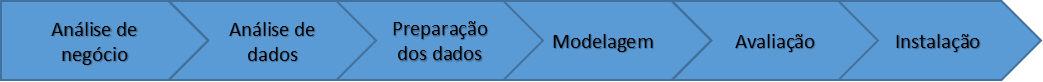
\includegraphics[scale=0.8]{img/CRISP-DM-main.png}
	\caption{Fases do CRISP-DM}
	\label{img:CRISP-DM-diagram}
\end{figure}

% Overview das fases 
%% p. 10-11
A seguir segue uma descrição breve de cada uma das fases:

\begin{enumerate}

\item \textbf{Análise do negócio}:
O objetivo desta fase é entender os requisitos e objetivos do projeto sob uma perspectiva de negócio, traduzí-los para requisitos e objetivos sob uma perspectiva de Mineração de Dados e então traçar um plano preliminar para alcançá-los.

\item \textbf{Análise dos dados}:
Esta fase inicia com uma coleta inicial de dados e segue para o estudo dos dados a fim de identificar problemas de qualidade, obter insights e detectar possíveis subconjuntos de dados que permitam desenvolver hipóteses sobre informações que não estejam presentes.

\item \textbf{Preparação dos dados}:
Esta fase é composta por atividades necessárias para gerar, a partir dos dados inicialmente coletados, um conjunto de dados a ser utilizado pelas ferramentas de modelagem. Inclui atividades como seleção de tabelas, registros, atributos, transformações e limpeza de dados.

\item \textbf{Modelagem}:
Nesta fase são aplicadas técnicas de modelagem e os modelos desenvolvidos são otimizados. Normalmente aplicam-se ao problema mais de uma técnicas de modelagem. Como algumas técnicas de modelagem podem exigir que os dados estejam em dado formato, pode ser necessário voltar para a fase Preparação dos dados.

\item \textbf{Avaliação}:
Esta fase é iniciada quando já foi desenvolvido um modelo com alta qualidade, do ponto de vista da Mineração de Dados. Nela são avaliados a adequação do modelo como ferramenta para alcançar o objetivo de negócio que motivou o projeto e a qualidade da instância do processo. Ela termina com a decisão pela utilização ou não dos resultados obtidos.

\item \textbf{Instalação}:\todo{qual a tradução para deployment?}
Após o desenvolvimento de um modelo, faz-se necessário que ele seja disponibilizado para os usuários finais, seja na forma de relatórios, seja na forma de sistemas de apoio à tomada de decisão, para que seja efetivamente utilizado, auxiliando no alcance dos objetivos de negócio que motivaram a criação do projeto.

\end{enumerate}

\newpage

\subsection*{1 - Análise do negócio}

% diagrama

\begin{figure}[H]
	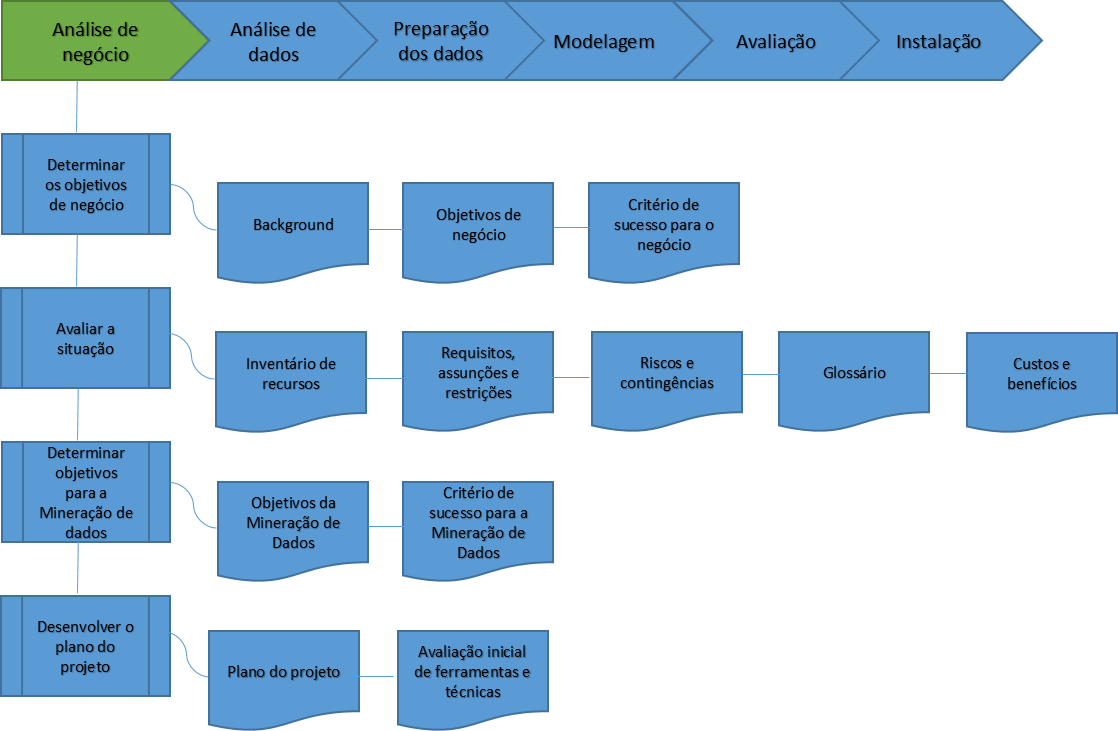
\includegraphics[scale=0.8]{img/CRISP-DM-Analise-de-negocio.png}
	\caption{Detalhamento da fase Análise de negócio}
	\label{img:CRISP-DM-analise-de-negocio}
\end{figure}

% Tarefas e saídas

\subsubsection*{\textbf{1.1 - Analisar os objetivos de negócio}}

O primeiro passo em um projeto de Mineração de Dados é analisar, sob uma perspectiva de negócio, o que realmente o cliente deseja alcançar. Normalmente o cliente possui vários objetivos concorrentes e restrições, que devem ser balanceados. O objetivo desta tarefa é descobrir fatores importantes do negócio que possam influenciar no resultado do projeto. Uma das consequências de se negligenciar esse passo é o projeto finalizar respondendo corretamente a perguntas erradas.

\subsubsection*{Background}

Registro das informações sobre o estado do negócio no início do projeto.

\subsubsection*{Objetivos do negócio}

Registra o objetivo primário do projeto, sob uma perspectiva de negócio, além de outras questões de negócio que o cliente objetiva esclarecer.

\subsubsection*{Critério de sucesso, sob uma perspectiva de negócio}

Registra os critérios para que o projeto seja considerado um sucesso, sob uma perspectiva de negócio.

\subsubsection*{\textbf{1.2 - Avaliar a situação}}

O objetivo desta tarefa é analisar mais detalhadamente de informações importantes para determinar os objetivos da Mineração de Dados e desenvolver um plano para o projeto. São analisadas informações como quais os recursos disponíveis, quais as restrições e quais as assunções.

\subsubsection*{Inventário de recursos}

Registra os recursos disponíveis para o projeto, como recursos humanos(especialistas do negócio, analistas de dados, técnicos de suporte), dados(arquivos, bases de dados operacionais, data warehouses), hardwares e softwares.

\subsubsection*{Requisitos, assunções e restrições}

Registra os requisitos do projeto, incluindo prazos, níveis de qualidade, segurança e aspectos legais.
Registra as assunções do projeto, sejam assunções que poderão ser verificadas a partir dos dados utilizados pelo projeto, sejam assunções que não poderão ser verificadas. No caso de assunções que não poderão ser verificadas, é importante que sejam registradas, principalmente caso possam afetar a validade dos resultados do projeto.
Registra as restrições do projeto, sejam restrições na disponibilidade de recursos, sejam restrições tecnológicas.

\subsubsection*{Riscos e planos de contingência}

Registra os eventos que, caso ocorram, poderão afetar os prazos ou a qualidade do projeto, bem como os planos de contingência, detalhando que ações devem ser executadas caso esses eventos ocorram.

\subsubsection*{Glossário}

Registra o conjunto de termos e seus significados que são relevantes para o projeto. Inclui tanto termos pertencentes à terminologia do negócio, quanto termos pertencentes à terminologia de Mineração de Dados.

\subsubsection*{Custos e benefícios}

Registra uma análise dos custos do projeto comparados com os potenciais benefícios para o negócio, caso o projeto alcance sucesso. Essa comparação deve ser o mais específico possível. Por exemplo, pode-se utilizar valores monetários em contextos comerciais.

\subsubsection*{\textbf{1.3 - Analisar os objetivos de Mineração de Dados}}

O objetivo desta tarefa é traduzir para objetivos, numa perspectiva de Mineração de Dados, os objetivos de negócio analisados na tarefa 1.1.

\subsubsection*{Objetivos da Mineração de Dados}

Registra os resultados objetivados pelo projeto para auxiliar no alcance dos objetivos de negócio.

\subsubsection*{Critério de sucesso, sob uma perspectiva de Mineração de Dados}

Registra, em termos técnicos, os critérios para determinar se o projeto alcançou sucesso.

\subsubsection*{\textbf{1.4 - Desenvolver um plano do projeto}}

Registra um plano para alcançar os objetivos de Mineração de Dados e então os objetivos de negócio. Inclui tanto as atividades a serem desenvolvidos, quanto as ferramentas e técnicas a serem utilizadas.

\subsubsection*{Plano do projeto}

Registra as atividades a serem desenvolvidas, incluindo duração, recursos necessários, entradas, saídas e dependências. É importante que sejam registradas as dependências e riscos das atividades e como podem impactar nos prazos.
Dado o aspecto iterativo de um projeto de Mineração de Dados, o plano de projeto é um documento dinâmico, sendo recomendado que ao fim de cada fase ele seja revisado e atualizado.

\subsubsection*{Avaliação inicial de ferramentas e técnicas}

Registra a avaliação de ferramentas e técnicas para a escolha de quais serão utilizadas no projeto. É importante que essa análise seja realizada no início do projeto, dado que a escolha das ferramentas e técnicas podem influenciar todo o resto do projeto.

\newpage 

\subsection*{2 - Análise dos dados}

% diagrama 

\begin{figure}[H]
	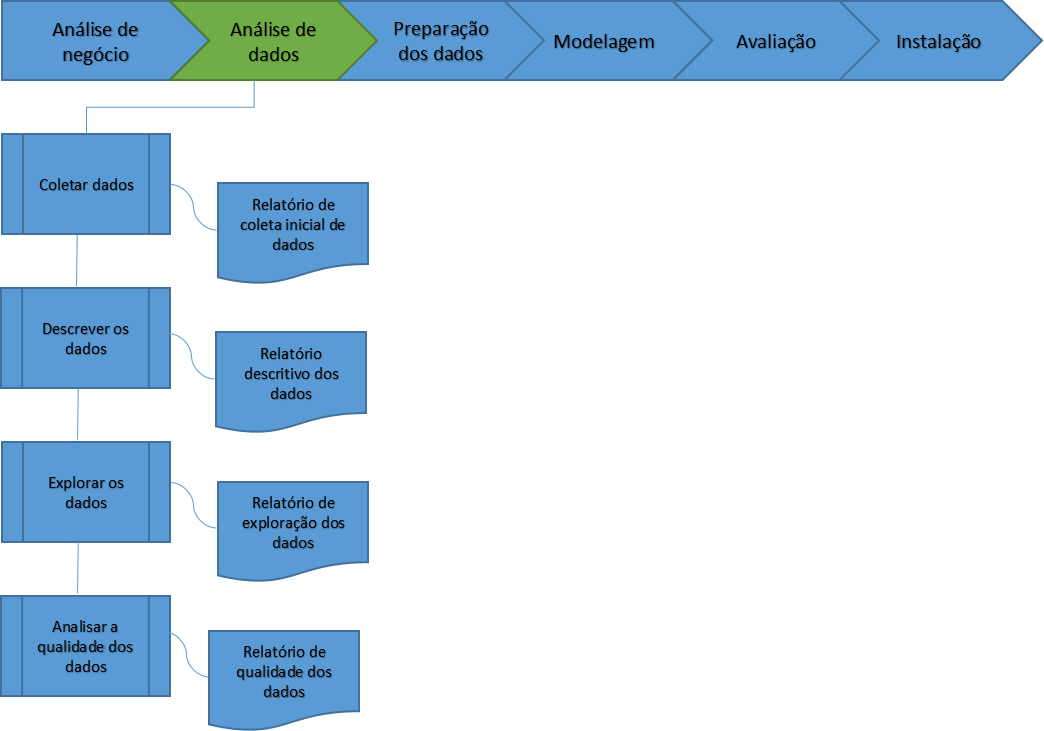
\includegraphics[scale=0.8]{img/CRISP-DM-Analise-dos-dados.png}
	\caption{Detalhamento da fase Análise dos dados}
	\label{img:CRISP-DM-Analise-dos-dados}
\end{figure}

% tarefas e saídas

\subsubsection*{\textbf{2.1 - Coletar dados}}

O objetivo desta tarefa é realizar a coleta dos dados indicados nos recursos do projeto. Nesta tarefa estão inclusos tanto o trabalho de extração quanto de integração dos dados, caso provenham de fontes de dados diferentes.

\subsubsection*{Relatório da coleta inicial de dados}

Registra os conjuntos de dados coletados, suas localizações, os métodos utilizados na coleta e problemas, com respectivas soluções adotadas, que nela tenham ocorrido.

\subsubsection*{\textbf{2.2 - Descrever os dados}}

O objetivo desta tarefa é realizar uma análise estrutural dos dados, avaliando se eles satisfazem os requisitos do projeto.

\subsubsection*{Relatório descritivo dos dados}

Registra informações sobre os dados coletados, como formato, quantidade de registros e nomes de atributos.

\subsubsection*{\textbf{2.3 - Explorar os dados}}

O objetivo desta tarefa é realizar uma análise da distribuição dos dados, através de consultas, visualizações e técnicas de report\todo{report techniques...}. Nela estão inclusas análise da distribuição de atributos dos dados, análise do relacionamento entre pares de atributos, análise de subpopulações e análise estatística. 

\subsubsection*{Relatório de exploração dos dados}

Registra as descobertas dessa tarefa e impacto que causarão no projeto.

\subsubsection*{\textbf{2.4 - Analisar a qualidade dos dados}}

O objetivo desta tarefa é analisar a qualidade dos dados, verificando, por exemplo, se são completos(há registros para todos os casos necessários), se são corretos(ausência de erros), se há dados ausentes; e analisar soluções para os problemas de qualidade encontrados.

\subsubsection*{Relatório de qualidade dos dados}

Registra os resultados da análise de qualidade dos dados, indicando, os problemas de qualidade e as possíveis soluções.

\newpage

\subsection*{3 - Preparação dos dados}

% diagrama

\begin{figure}[H]
	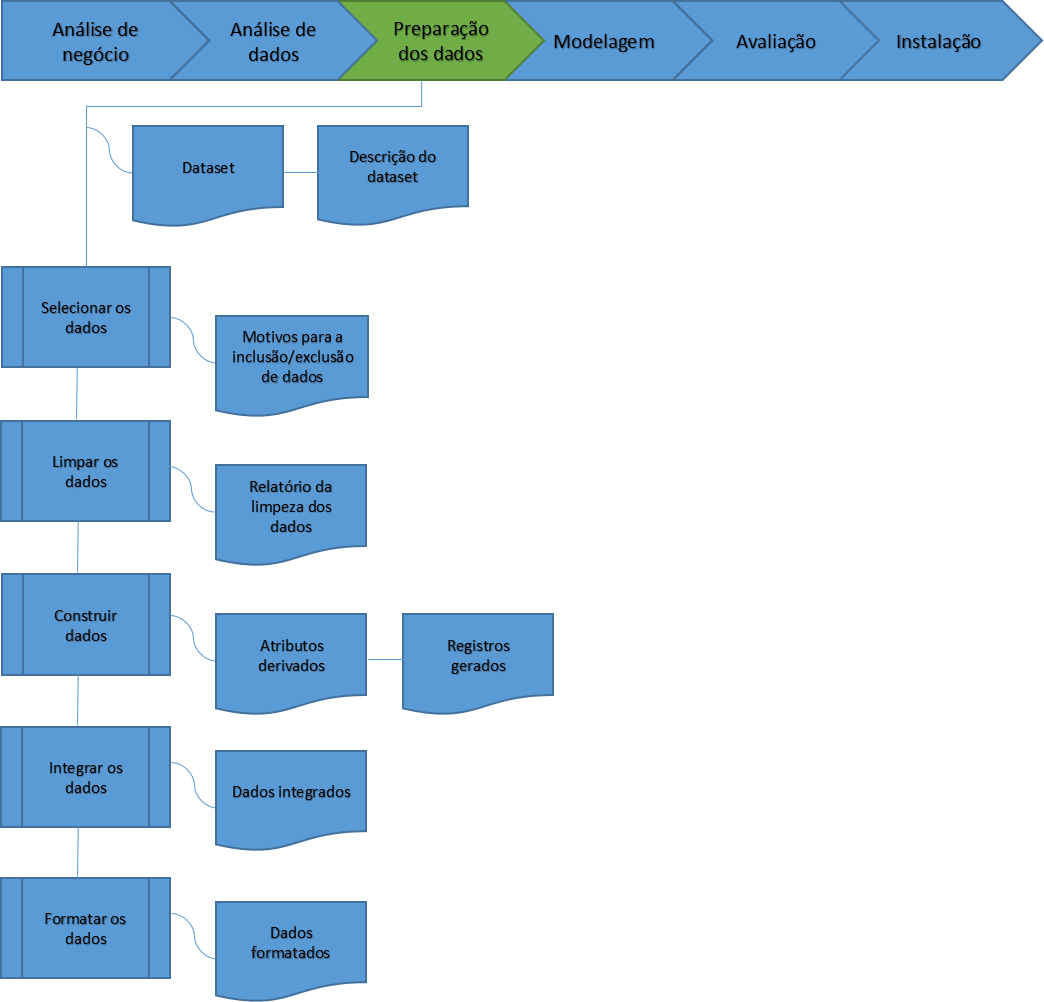
\includegraphics[scale=0.8]{img/CRISP-DM-Preparacao-dos-dados.png}
	\caption{Detalhamento da fase Preparação dos dados}
	\label{img:CRISP-DM-Preparacao-dos-dados}
\end{figure}

% tarefas e saídas

\subsubsection*{Dataset}

Datasets produzidos por esta fase, a serem utilizados no desenvolvimento de modelos ou em análises.

\subsubsection*{Descrição do dataset}

Registra informações sobre o dataset produzido por esta fase.

\subsubsection*{\textbf{3.1 - Selecionar dados}}

O objetivo desta tarefa é selecionar um subconjunto de dados a serem utilizados nas análises posteriores. Essa seleção envolve tanto a seleção de registros quanto a seleção de atributos. A lista de critérios para essa seleção inclui relevância dos dados para os objetivos de Mineração de Dados, qualidade e restrições técnicas, como limite no volume dos dados ou nos tipos dos dados.

\subsubsection*{Motivos para inclusão/exclusão de dados}

Registra os motivos para inclusão e exclusão de dados.

\subsubsection*{3.2 - Limpar os dados}

O objetivo desta tarefa é produzir um dataset com nível de qualidade adequado para a aplicação das técnicas e modelos selecionados pelo projeto, resolvendo os problemas de qualidade analisados na tarefa Analisar a qualidade dos dados. Para tanto, atividades como seleção de subconjunto dos dados, inserção de valores default e estimação de valores ausentes poderão ser necessárias.

\subsubsection*{Relatório da limpeza dos dados}

Registra as alterações realizadas nos dados para resolver problemas de qualidade, indicando os motivos e possíveis consequências.

\subsubsection*{\textbf{3.3 - Construir dados}}

O objetivo desta tarefa é a criação de novos dados, sejam derivados de dados já existentes, sejam novos registros, criados, por exemplo, através de interpolação de outros registros já existentes.

\subsubsection*{Atributos derivados}

Registra os atributos que foram construídos a partir de outros já existentes. Por exemplo, área = altura * largura.

\subsubsection*{Registros gerados}

Registra a geração de novos registros. 

\subsubsection*{\textbf{3.4 - Integrar os dados}}

O objetivo desta tarefa é criar novos dados através da integração de dados de fontes diversas.

\subsubsection*{Dados integrados}

Esta saída é composta tanto pelos dados que foram gerados a partir da integração de dados de fontes diversas, quanto dados agregados.

\subsubsection*{\textbf{3.5 - Formatar os dados}}

O objetivo desta tarefa é realizar transformações nos dados que não alterem seus significados, necessárias para que os dados possam ser utilizados pelas ferramentas. Exemplos de transformações são mudança do formato do arquivo onde estão os dados, alteração na ordem das colunas ou alteração na ordem dos registros.

\subsubsection*{Dados formatados}

Registra as transformações realizadas nos dados, indicando motivos e possíveis consequências.

\newpage 

\subsection*{4 - Modelagem}

% diagrama

\begin{figure}[H]
	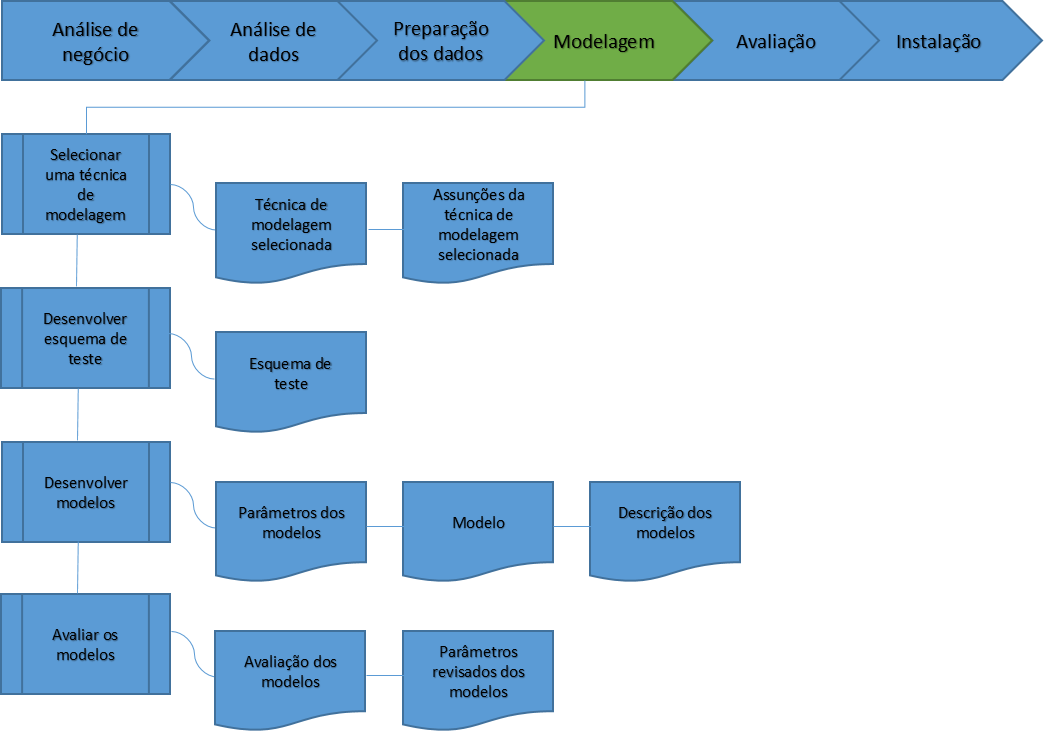
\includegraphics[scale=0.8]{img/CRISP-DM-Modelagem.png}
	\caption{Detalhamento da fase Modelagem}
	\label{img:CRISP-DM-Modelagem}
\end{figure}

% tarefas e saídas

\subsubsection*{\textbf{4.1 - Selecionar uma técnica de modelagem}}

O objetivo desta tarefa é selecionar uma técnica de modelagem a ser aplicada a um dataset gerado. No caso de várias técnicas de modelagem terem sido escolhidas para serem aplicadas, esta tarefa deve ser executada para cada uma delas.

\subsubsection*{Técnica de modelagem selecionada}

Registra informações sobre a técnica de modelagem selecionada.

\subsubsection*{Assunções da técnica de modelagem selecionada}

Registra as assunções feitas pela técnica de modelagem selecionada. Por exemplo, que todos os registros são independentes ou que todos os atributos possuem distribuição uniforme.

\subsubsection*{\textbf{4.2 - Desenvolver esquema de teste}}

O objetivo desta tarefa é desenvolver um procedimento ou mecanismo para testar a qualidade e validade do modelo a ser desenvolvido. Para tanto, deve-se decidir, por exemplo, sobre como os dados serão particionados em subconjuntos de treinamento e de teste e quais métricas serão utilizadas para avaliar o desempenho.

\subsubsection*{Esquema de teste}

Registra um plano para treinamento, teste e avaliação do modelo a ser desenvolvido.

\subsubsection*{\textbf{4.3 - Desenvolver modelos}}

O objetivo desta tarefa é aplicar a técnica de modelagem escolhida ao dataset desenvolvido na fase anterior.

\subsubsection*{Parâmetros dos modelos}

Registra os parâmetros utilizados pelos modelos desenvolvidos, bem como os motivos para suas escolhas.

\subsubsection*{Modelos}

Modelos desenvolvidos.

\subsubsection*{Descrição dos modelos}

Registra informações sobre os modelos desenvolvidos, como, por exemplo, como interpretá-los.

\subsubsection*{\textbf{4.4 - Avaliar os modelos}}

O objetivo desta tarefa é avaliar os modelos desenvolvidos sob uma perspectiva de Mineração de Dados, verificando se os critérios de sucesso de Mineração de Dados foram satisfeitos, se os resultados do testes foram satisfatórios. Os modelos desenvolvidos devem ser então comparados e ordenados de acordo com critérios de avaliação.

\subsubsection*{Avaliação dos modelos}

Registra os resultados da tarefa Avaliar o modelo, como a performance dos modelos desenvolvidos e uma ordem dos modelos de acordo com critérios de qualidade.

\subsubsection*{Parâmetros revisados dos modelos}

Registra alterações propostas em parâmetros dos modelos desenvolvidos de acordo com a avaliação dos modelos. Os parâmetros revisados servem para serem utilizados no desenvolvimento, em uma nova iteração, de novos modelos.

\newpage 

\subsection*{5 - Avaliação}

% diagrama

\begin{figure}[H]
	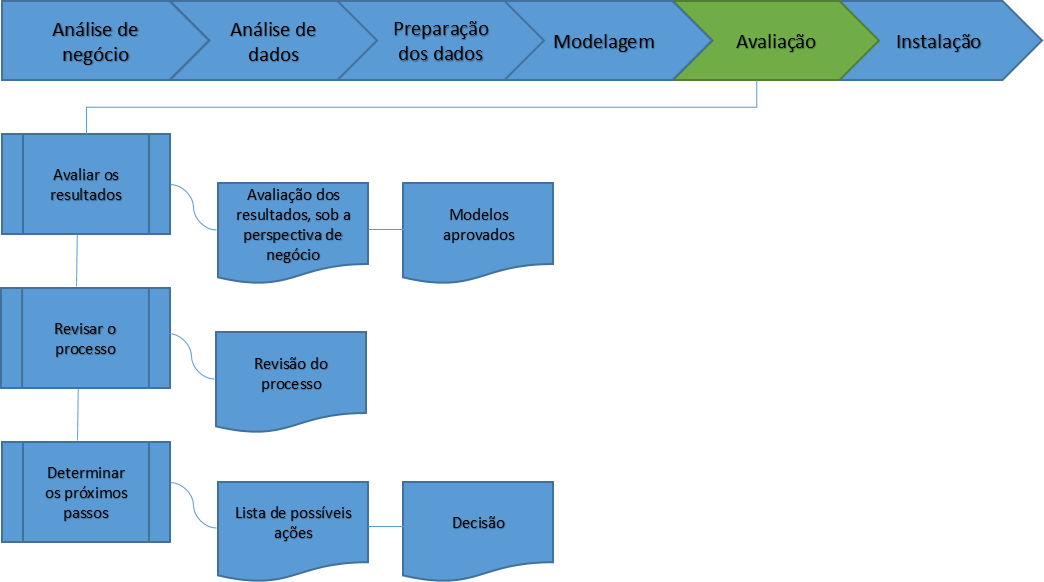
\includegraphics[scale=0.8]{img/CRISP-DM-Avaliacao.png}
	\caption{Detalhamento da fase Avaliação}
	\label{img:CRISP-DM-Avaliacao}
\end{figure}

% tarefas e saídas

\subsubsection*{\textbf{5.1 - Avaliar os resultados}}

O objetivo desta tarefa é avaliar em que medida os resultados alcançados com a Mineração de Dados, sejam modelos desenvolvidos, sejam informações extraídas, auxiliam no alcance dos objetivos de negócio e, se possível, testar os modelos desenvolvidos em aplicações reais.

\subsubsection*{Avaliação dos resultados, sob a perspectiva de negócio}

Registra a avaliação dos resultados, indicando se o projeto obteve sucesso em suportar os objetivos de negócio.

\subsubsection*{Modelos aprovados}

Conjunto de modelos que na avaliação dos resultados apresentaram resultados satisfatórios.

\subsubsection*{\textbf{5.2 - Revisar o processo}}

A partir deste ponto do processo os modelos desenvolvidos já apresentam resultados satisfatórios e torna-se apropriada a realização de uma revisão do processo, a fim de verificar a qualidade das atividades até então desenvolvidas.

\subsubsection*{Revisão do processo}

Registra os resultados da revisão do processo, indicando atividades que não foram desenvolvidas com a qualidade esperada e que deverão ser repetidas.

\subsubsection*{\textbf{5.3 - Determinar os próximos passos}}

O objetivo desta tarefa é definir quais as próximas atividades a serem desenvolvidas, de acordo com os resultados da avaliação dos resultados, da revisão do processo e dos recursos disponíveis para o projeto. Pode-se decidir pela implantação dos modelos desenvolvidos, pela realização de uma nova iteração ou a finalização do projeto.

\subsubsection*{Lista de possíveis ações}

Registra as potenciais ações a serem executadas e os respectivos motivos para execução ou não.

\subsubsection*{Decisão}

Registra a decisão sobre quais os próximos passos a serem seguidos e a respectiva motivação.

\newpage 

\subsection*{6 - Instalação}

% diagrama

\begin{figure}[H]
	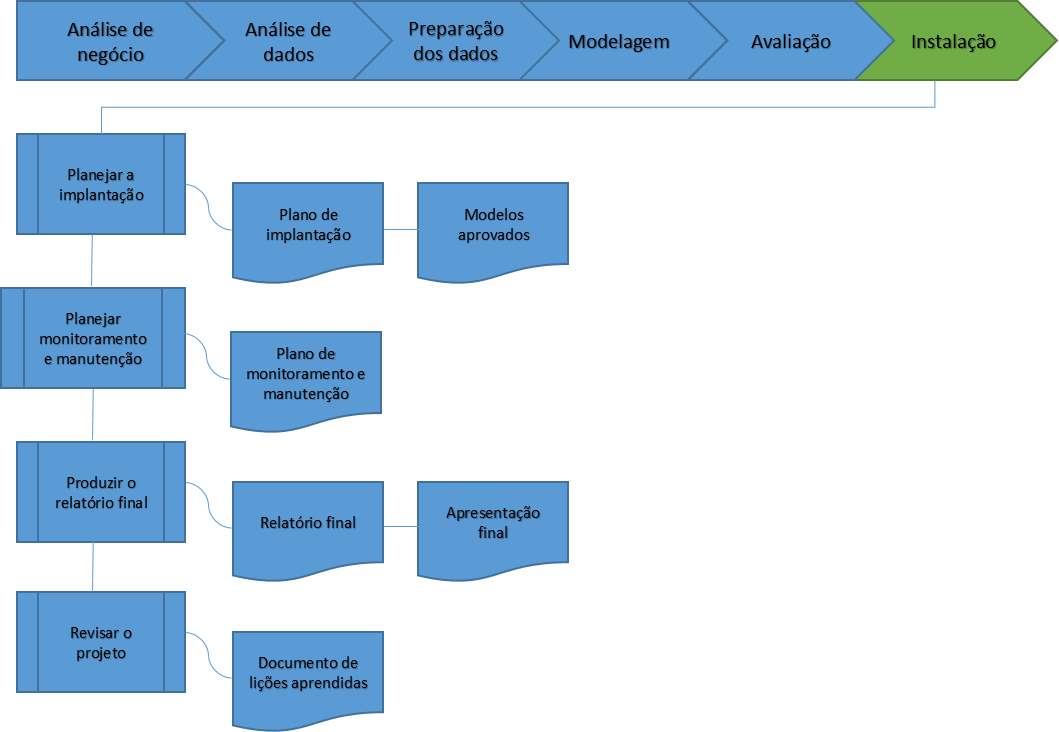
\includegraphics[scale=0.8]{img/CRISP-DM-Implantacao.png}
	\caption{Detalhamento da fase Implantação}
	\label{img:CRISP-DM-Implantação}
\end{figure}

% tarefas e saídas

\subsubsection*{\textbf{6.1 - Planejar a implantação}}

O objetivo desta tarefa é produzir um plano de implantação dos modelos aprovados.

\subsubsection*{Plano de implantação}

Registra as atividades necessárias para a implantação dos modelos aprovados.

\subsubsection*{\textbf{6.2 - Planejar monitoramento e manutenção}}

O objetivo desta tarefa é desenvolver planos de monitoramento e manutenção, objetivando verificar os resultados dos modelos implantados e evitar que sejam utilizados indevidamente ou tornem-se obsoletos.

\subsubsection*{Plano de monitoramento e manutenção}

Registra as estratégias de monitoramento e de manutenção.

\subsubsection*{\textbf{6.3 - Produzir relatório final}}

O objetivo desta tarefa é produzir um relatório registrando um histórico do projeto.

\subsubsection*{Relatório final}

Registra um histórico do projeto.

\subsubsection*{Apresentação final}

Apresentação dos resultados alcançados pelo projeto.

\subsubsection*{\textbf{6.4 - Revisar o projeto}}

O objetivo desta tarefa é analisar o que foi feito correta e incorretamente no projeto.

\subsubsection*{Documento de lições aprendidas}

Registra as lições aprendidas no projeto, indicando que ações foram executadas corretamente, para que sejam reforçadas, e que ações foram executadas incorretamente, para que sejam corrigidas em futuros projetos.

\section{Ferramentas utilizadas}